% !TeX root = ../../thesis.tex
\chapter{Introduction}\label{ch:introduction}

% \instructionsintroduction

% Illustration on how to refer to your papers when using biblatex
% (see second line in thesis.tex to activate biblatex)
%\definecolor{shadecolor}{gray}{0.85}
%\begin{shaded}
%This chapter was previously published as:\\
%\fullcite{VandenBroeck2011IJCAI}
%\newpage
%\end{shaded}

\section{Phylogenetics}

\cite{FrRo2010Diffusion}

\section{Bayesian statistics}

\section{Bayesian phylodynamics and joint inference}

Bayesian statistics and MCMC are good for phylogenies.
We can gibbs sample anything.. idk..


\section{Viral pathogens}

Viral pathogens are a particularly useful study system for Bayesian phylogeneticists because their small genomes and fast evolutionary rate facilitate both tractable computation and a constant stream of constantly evolving genomes.
Addditionally, viruses frequently cause human suffering and death, both as endemic diseases (seasonal influenza, hepatitis, etc.) and the agents behind sudden disease epidemics (Zika, Ebola, Lassa).
Indeed, viruses have been responsible for the majority of the most deadly pandemics of the last century (Spanish influenza, tons of other flu pandemics, Covid).
Like, do I really need to convince you, dear reader?
The whole world has been locked in their houses for the last two months for gods sake.

\subsection{Zika Virus}

\subsection{Hepatitis B Virus}

\subsection{Lassa Virus}


% Some dummy code to get at least 1 entry in the nomenclature.
% \nomenclature{$\Theta$}{A nice symbol}
% Introducing some symbol: $\Theta$.

% Some dummy code to get at least 1 entry in the list of
% abbreviations.
\newglossaryentry{beast}{name={BEAST},description={Bayesian Evolutionary Analysis Sampling Trees}}
Introducing an acronym: \gls{beast}.

% Some dummy code show how to include images.
% \begin{figure}
%   \centering
%   \medskip
%   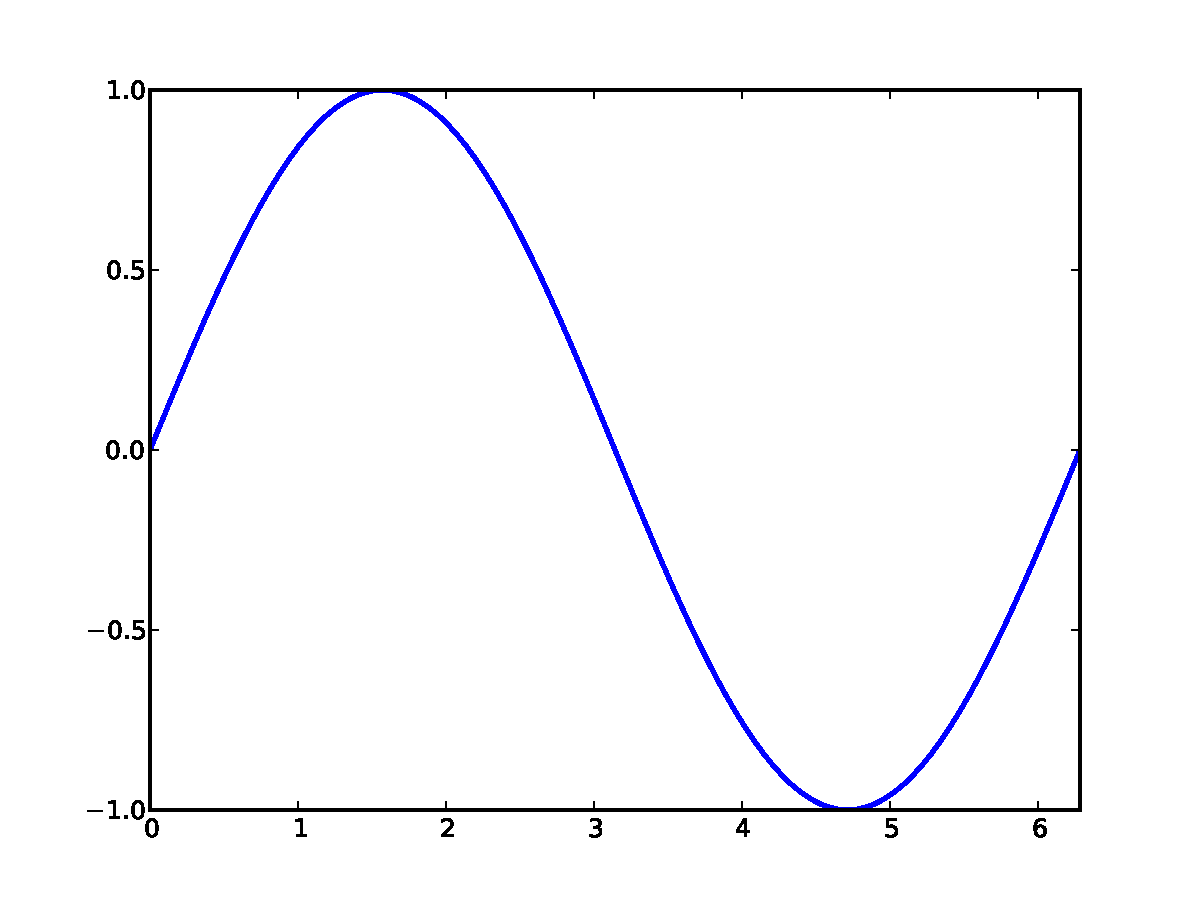
\includegraphics[width=.9\textwidth]{sine}
%   \caption[Short caption for Table of Figures]{Illustration of how to
%   include a figure (long text, should not go to Table of Figures).}
%   \label{fig:sine}
% \end{figure}





%%%%%%%%%%%%%%%%%%%%%%%%%%%%%%%%%%%%%%%%%%%%%%%%%%
% Keep the following \cleardoublepage at the end of this file,
% otherwise \includeonly includes empty pages.
\cleardoublepage

% vim: tw=70 nocindent expandtab foldmethod=marker foldmarker={{{}{,}{}}}
